\documentclass[12pt]{article}
\usepackage[margin=1.0in]{geometry} %page layout
\usepackage[usenames,dvipsnames]{color} %color
\definecolor{light-gray}{gray}{0.95}
\definecolor{darkgreen}{rgb}{0,0.4,0}
\usepackage{graphicx, subfigure} %figures
\usepackage{url, hyperref} %cross-referencing
\usepackage{amsmath, amssymb} %math
\usepackage{listings} %source code
\lstset{breaklines=true,
breakindent=0pt,
prebreak=\mbox{\tiny$\searrow$},
postbreak=\mbox{{\color{blue}\tiny$\rightarrow$}},
numbers=left,
commentstyle=\color{darkgreen},
numberblanklines=false,
frame=single,
captionpos=b,
backgroundcolor=\color{light-gray}}
\usepackage[3D]{movie15} %for movies (needs hyperref)
	\newenvironment{changemargin}[2]
	{
	  	\begin{list}{}
		{
			\setlength{\topsep}{0pt}%
			\setlength{\leftmargin}{#1}%
			\setlength{\rightmargin}{#2}%
			\setlength{\listparindent}{\parindent}%
			\setlength{\itemindent}{\parindent}%
			\setlength{\parsep}{\parskip}%
		}
	  	\item[]
		}
		{\end{list}
	}
\author{Salman Aslam\\Georgia Tech}
\title{RVQ Experiments}
\author{Salman Aslam\\ Georgia Institute of Technology}
\date{}
\definecolor{darkgreen}{rgb}{0,0.5,0}
\newcommand{\Ntrg}{\big[N_{t=1, m=1} + \lambda \big] + \big[N_{t=1, m=2} + \lambda \big] + \ldots + \big[N_{t=1, m=M} + \lambda \big]}
\newcommand{\jointcnt}{\sum\limits_{n_{trg}=1}^{N_{trg}}I(X_t=x_t, X_{t-1}=x_{t-1})}
\newcommand{\singlecnt}{\sum\limits_{n_{trg}=1}^{N_{trg}}I(X_{t-1}=x_{t-1})}
\newcommand{\singlep}{p(X_{t-1}=x_{t-1})}
\newcommand{\singlepone}{p(X_{t-1}=1)}
\newcommand{\singleptwo}{p(X_{t-1}=2)}
\newcommand{\singlepM}{p(X_{t-1}=M)}
\newcommand{\condp}{p(X_t=x_t | X_{t-1}=x_{t-1})}
\newcommand{\jointp}{p(X_t=x_t, X_{t-1}=x_{t-1})}
\newcommand{\KmeansOuterSum}{\sum\limits_{k=1}^K}
\newcommand{\KmeansInnerSum}{\sum\limits_{{i=1 \atop x_i \in \mathcal{K}_k}}^N}
\newcommand{\KmeansSum}{\KmeansOuterSum \KmeansInnerSum}
\newcommand{\RVQInnerSum}{\sum\limits_{{i=1 \atop g_i \mapsto m_{\tau, s}}}^N}
\newcommand{\RVQOuterSum}{\sum_{s=1}^S}
\newcommand{\RVQsum}{\KmeansOuterSum \sum\limits_{{i=1 \atop g_i \in \mathcal{K}_k}}^N}
\newcommand{\KmeansInner}{{(x_i - \mu_k)}^2}
\newcommand{\RVQinner}{            {(x_i  - \hat{\mu}^{(k)})}^2}
\newcommand{\RVQinneralternate}{{(g_i - m_\tau^{(k)})}^2}
\newcommand{\RVQinneralternatealternate}{{(g_i - m_{\tau, s})}^2}
\newcommand{\KmeansError}{\KmeansSum \KmeansInner}
\newcommand{\RVQerror}     {\KmeansSum \RVQinner}
\newcommand{\RVQerroralternate}{\RVQsum \RVQinneralternate}
\newcommand{\RVQunit}{x_i -\bigg(\sum_{t=1}^Tm^{(k)}_t\bigg)}
\newcommand{\RVQequivalentCodevector}{\sum_{t=1 }^Tm^{(k)}_t}
\newcommand{\RVQequivalentCodevectorBroken}{\sum_{t=1 \atop t \neq \tau}^Tm^{(k)}_t+ m^{(k)}_\tau}
\newcommand{\RVQmultipleKmeans}{x_i -\bigg(\RVQequivalentCodevectorBroken\bigg)}
\newcommand{\RVQmultipleKmeansone}{x_i -\sum_{t=2}^Tm^{(k)}_t+ m^{(k)}_1\bigg)}
\newcommand{\RVQmultipleKmeansonealternate}{\bigg(x_i -\sum_{t=1 \atop t \neq \tau}^Tm^{(k)}_t\bigg) - m^{(k)}_\tau}
\newcommand{\RVQmultipleKmeanstwo}{x_i -\bigg(\sum_{t=1 \atop t \neq 2}^Tm^{(k)}_t+ m^{(k)}_2\bigg)}
\newcommand{\RVQmultipleKmeansT}{x_i -\bigg(\sum_{t=1}^{T-1}m^{(k)}_t+ m^{(k)}_2\bigg)}
\newcommand{\EucMatrix}
{
\left[
\begin{array}{lll}
r_{11} & r_{12} & t_x \\ 
r_{21} & r_{22} & t_y \\ 
0 & 0 & 1 \\ 
\end{array}
\right]
}	

\newcommand{\SimMatrix}
{
\left[
\begin{array}{lll}
sr_{11} & sr_{12} & t_x \\ 
sr_{21} & sr_{22} & t_y \\
0 & 0 & 1 \\ 
\end{array}
\right]
}

\newcommand{\AffMatrix}
{
\left[
\begin{array}{lll}
a &b & t_x \\ 
c & d & t_y \\
0 & 0 & 1 \\
\end{array}
\right]
}

\newcommand{\ProjMatrix}
{
\left[
\begin{array}{lll}
h_{11} & h_{12} & h_{13} \\ 
h_{21} & h_{22} & h_{23} \\ 
h_{31} & h_{32} & h_{33} \\ 
\end{array}
\right]
}

\newcommand{\RotMatrixTheta}
{
\left[
\begin{array}{rr}
\cos(\theta) & -\sin(\theta) \\ 
\sin(\theta) & \cos(\theta) \\ 
\end{array}
\right]
}

\newcommand{\RotMatrixPhi}
{
\left[
\begin{array}{rr}
\cos(\phi) & -\sin(\phi) \\ 
\sin(\phi) & \cos(\phi) \\ 
\end{array}
\right]
}

\newcommand{\RotMatrixminusPhi}
{
\left[
\begin{array}{rr}
\cos(-\phi) & -\sin(-\phi) \\ 
\sin(-\phi) & \cos(-\phi) \\ 
\end{array}
\right]
}


\newcommand{\EigenvalueMatrix}
{
\left[
\begin{array}{cc}
\lambda_1 & 0\\
0 & \lambda_2
\end{array}
\right]
}

\newcommand{\bigMatrix}
{
s \left[
\begin{array}{cc}
 (r)(a) + b &  (r)(d) - c \\
 (r)(c) - d &  (r)(b) + a
\end{array}
\right]
}


\newcommand{\bigMatrixTwo}
{
\left[
\begin{array}{cc}
(\lambda_2) p + (\lambda_1) q & (\lambda_2) s  - (\lambda_1) r \\
(\lambda_2) r  - (\lambda_1) s & (\lambda_2) q + (\lambda_1) p
\end{array}
\right]
}
\newcommand{\dr}{(\mathbf{x}_i-\boldsymbol\mu_k)^T(\mathbf{x}_i-\boldsymbol\mu_k) + \lambda({Q_{\textrm{max}}-Q_i})}

\begin{document}
\maketitle
\rule[0pt]{\textwidth}{1pt}
\tableofcontents
\rule[0pt]{\textwidth}{1pt}

%================================
\section{Introduction}
%================================
Our goal is to examine the effects on training and test error of varying $q$, the number of stages in RVQ, while keeping $m$, the number of code-vectors per stage fixed.  For this, we train an 8x4 RVQ (maximum q=8, m=4) using four different data distributions in $\mathbb{R}^{1089}$: (a) Dudek sequence, (b) Uniform random variable, (c) Gaussian random variable, and (d) Gauss-Markov random variable.

%================================
\section{Theory}
%================================
While examining the effects on training and test error of varying $q$, we would also like to relate the notions of generalization ability of RVQ, varying $q$ and VC dimension in statistical learning theory.  The  motivation behind this is to get a theoretical justification for using a particular $q$ in a given situation.  In particular, this is given by the notion of empirical risk minimization.

The concept of VC dimension was introduced by Vapnik~\cite{1999_BOOK_PRML_Vapnik} as a means of specifying the generalization ability of classifiers.  In this work, we look at some definitions leading up to the VC dimension.  It has been shown that the VC dimension of a nearest neighbor classifier is equal to the number of reference points in the training set~\cite{2003_JNL_PRML_Karacali}.  We extend this to show that the VC dimension of an RVQ classifier depends on both its number of stages $Q$ and the number of code-vectors per stage $M$.


In pattern recognition, a \emph{classifier} $g(x)$ is a function that maps $x_i \in \mathbb{R}^D$ to a set of $M$ discrete \emph{class} labels, $\theta  \in \{1, 2, \ldots M\}$, i.e., $g(x):~\mathbb{R}^D~\rightarrow~\{1, 2, \ldots M\}$.  The classifier errs if $g(x) \neq \theta$~\cite{1996_BOOK_PR_DevroyeGyorfiLugosi}.  Since it is not possible to create a classifier that always achieves perfect mapping, we create a probabilistic setting and let $\mathbf{X} \times \mathbf{\Theta}$ be an $\mathbb{R}^D \times \{1, 2, \ldots M\}$-valued random pair.  

\begin{enumerate}
\item \underline{Risk}.  The probability of error for estimator $g(x)$, the {\color{blue}\emph{risk}} is

\begin{equation}
\boxed{
{\color{blue}R(g)} = \mathbf{P}(g(\mathbf{X}) \neq \mathbf{\Theta})}
\label{Eqn:loss}
\end{equation}

\item \underline{Bayes Risk}. In Equation~\ref{Eqn:loss}, the minimal probability of error $\mathbf{P}^*$ is called the \emph{Bayes error} or the \emph{Bayes risk}.  

\item \underline{Bayes Classifier}.  In Equation~\ref{Eqn:loss}, the best classifier $g^*$ is called the \emph{Bayes classifier} or the \emph{Bayes rule}, and is given by

\begin{equation}
g^* = \arg\min_{\tiny g:~\mathbb{R}^D~\rightarrow~\{1, 2, \ldots M\}} {\color{blue}R(g)}
\end{equation}

\item \underline{Empirical risk}. In practical situations, $\mathbf{P}(g(\mathbf{X}) \neq \mathbf{\Theta})$ is generally unknown, and therefore so is $g^*$.  However, we assume that we have $N$ i.i.d. random pairs of training data, $\{(x_1, \theta_1), (x_2, \theta_2), \ldots, (x_N, \theta_N)\}$ with the same distribution as $p(\mathbf{X},\mathbf{\Theta})$.  The empirical risk function for this data is $R_N$, or $R(g_N)$~\footnote{The quantity $\mathbb{E}\left[R_N\right]$ is marginally useful since it is the quality of an average data sequence and not the data sequence at hand.  A \emph{consistent} classifier is one for which $\lim\limits_{N \rightarrow \infty}\mathbb{E}\left[R_N\right] = R^*$~\cite{1996_BOOK_PR_DevroyeGyorfiLugosi}.}.
  
\item \underline{Empirical risk minimization}.
Since we cannot find $g^*$, we change the setting and define $R$ as being the risk of the best classifier in class $\mathcal{C}$, for instance, all $k$-nearest neighbor classifiers with all possible values of $k$.  Then,

\begin{equation}
R \triangleq \inf\limits_{g_N \in \mathcal{C}} \mathbf{P}(g_N(\mathbf{X}) \neq \mathbf{\Theta})
\end{equation}

Using \emph{empirical risk minimization}~\cite{1999_BOOK_PRML_Vapnik}, we select a classifier $g_N$ from a class $\mathcal{C}$ by minimizing, 

\begin{equation}
\frac{1}{N} \sum\limits_{n=1}^N I_{g_N(x_n \neq \theta_n)}
\end{equation}

then the corresponding risk $R_N$ satisfies the following inequality for all $\epsilon > 0$

\begin{equation}
\mathbf{P}(R_N > R + \epsilon) \leq 8(N^h + 1) e^{-N\epsilon^2/128}
\end{equation}

where $h$ is the Vapnik Chervonenkis (VC) dimension.  The concept of VC dimension is related to \emph{shattering}.

\item \underline{Shattering}.  In the two-class classification problem, a given set of $N$ points can be labeled in $2^N$ ways.  If, for all possible labelings, a classifier $g(x)$ from the class $\mathcal{C}$ can be found which correctly assigns those labels, then we say that the set of $N$ points is shattered by the class $\mathcal{C}$~\cite{1998_JNL_SVM_Burges}.  An example of shattering in $\mathbb{R}^2$ is given in Figure~\ref{fig:shattering}.

\item \underline{VC dimension}.  If a classifier class $\mathcal{C}$, such as the class of linear classifiers, or the class of $k$-nearest neighbors with different values of $k$, has VC dimension $h$, then there exists at least one set of $h$ points that can be shattered by it, but in general, not every set of $h$ points can be shattered by the class~\cite{1998_JNL_SVM_Burges}.  For instance, in Figure~\ref{fig:shattering}, three collinear points cannot be shattered by a line.  One motivation to use the VC dimension is that it can be used to place a bound on test error given training error.  For $N$ training examples, the following bound holds with probability $1-\eta$\cite{1999_BOOK_PRML_Vapnik}:

\begin{equation}
R_{tst} \leq R_{trg} + \sqrt\frac{h(\log (2N/h)+1) - \log (\eta/4)}{N}
\end{equation}

This is a loose bound since it is over all possible distributions.  However, in many cases, for a given distribution, the actual bound is tighter~\cite{Videolectures.net}.

\item \underline{Nearest neighbor classifier}.  The most popular nonparametric classifier is the nearest neighbor classifier that assigns the class label of the nearest neighbor in the training set to unknown data~\cite{2003_JNL_PRML_Karacali}.  For the nearest neighbor rule, for all distributions, the risk $R_{1NN}$ is bounded above by twice the Bayes risk,

\begin{equation}
\lim\limits_{N \rightarrow \infty} \sup\mathbb{E}\left[R_{1NN}\right] \leq 2R^*  
\end{equation}

In this sense, half of the available information in an infinite collection of classified samples is contained in the nearest neighbor~\cite{1967_JNL_PRML_Cover}.  This provides strong motivation to use the 1NN classifier.  Moreover, it has been shown to work well under several situations~\cite{1996_BOOK_PR_DevroyeGyorfiLugosi}.

								\begin{figure}[t]
								\centering
								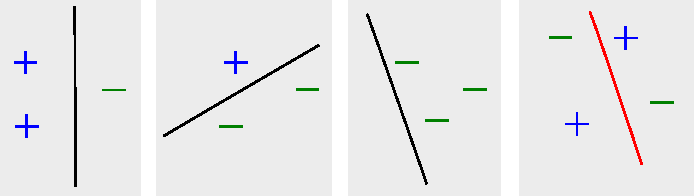
\includegraphics[width=1.0\textwidth]{figs/theory_PRML_shattering.pdf}
								\caption{A linear classifier in $\mathbb{R}^D$ can shatter $D+1$ points.  Here, in the first 3 examples, a line in $\mathbb{R}^2$ is able to shatter 3 points.  However, in the fourth example, it is unable to shatter 4 points.}
								\label{fig:shattering}
								\end{figure}

\item \underline{VC dimension of NN classifier}.   It has been shown by Kara\c{c}ali and Krim~\cite{2003_JNL_PRML_Karacali} that the VC dimension of the NN classifier is given by the number of reference points in the training set~\cite{2005_CNF_ML_Angiulli}.  These reference points can be obtained from the codevectors of a VQ codebook, such as an RVQ codebook.  For an RVQ codebook with $Q$ stages, and $M$ code-vectors per stage, there are $M^Q$ equivalent code-vectors.  Moreover, the number of direct-sum code-vectors at the end of the $q$-th stage is $M^q$\footnote{This assumes that there are no null code-vectors, i.e. code-vectors in which all elements are 0.}.   Therefore, the VC dimension of an RVQ nearest neighbor classifier in a variable-rate framework depends on how many stages and codevectors per stage are used.  Changing these numbers can be used to change the VC dimension of the RVQ NN classifier, and hence its generalization ability.  
\end{enumerate}

 


%================================
\section{Experiments}
%================================
In the following experiments, we keep $m$, the number of code-vectors per stage constant and vary $q$, the number of stages.  We see that as stages increase, the training error tends to decrease and so does test error, a sign of increasing VC dimension.

We make the following observations in Figure~\ref{fig:RVQ_results}:

\begin{itemize}
\item Training error decreases monotonically for eRMSE and dRMSE.
\item dRMSE is lower than eRMSE since the decoder is subject to one constraint while the encoder is subject to two.
\item Test error is always larger than training error.
\item For the Dudek experiment
\begin{itemize}
\item The error levels out after about 4 stages telling us that by about q=4, we are able to explain the statistical correlations in the data.  
\item RofE tends to further decrease in error after 5th stage telling us that the test snippet is a lot like the training snippet.  
\item maxQ which is forced to go all the way tells us, as mentioned in~\cite{1996_JNL_AdvancesRVQ_Barnes}, that using more stages in decoding will in many cases decrease rmse even if there are slight "bumps", i.e. increases in rmse along the way.  
\item monR, the greedy approach has highest rmse.
\item The curve has the "knee" that one would expect with a classifier as one increases the DoF.
\item At level 5, we see that there is clearly an increase in rms error which is why monR and nulE level out (monR exits but I continue showing its exit rmse), nulE rides out the wave and in the last stage is able to decrease rms error by another 0.0062.
\item maxQ and RofE take the very small increases in rms error, since they're not greedy, and are rewarded with gains as they use more and more stages.
\end{itemize}
\item The reconstruction error for the Gaussian and uniform random variables is almost constant since adding stages cannot explain a test example that is statistically independent of the training data.  We see the same behavior in PCA and TSVQ as well.
\item For the Gauss-Markov example, the statistical correlation is captured in about 2 stages.
\item Of the random variable experiments, the highest reconstruction errors are for Gaussian, uniform and Gauss-Markov random variables, as expected.  The reason is that the Gaussian distribution has the highest entropy, followed by the uniform random variable, and then followed by the statistically correlated Gauss-Markov random variable.
\end{itemize}

\begin{figure}
\subfigure[Dudek sequence, a 100 33x33 ($\mathbb{R}^{1089}$) face snippets were extracted from the first 100 images and used as training examples.  The test example is a single 33x33 snippet from the 101st image.]{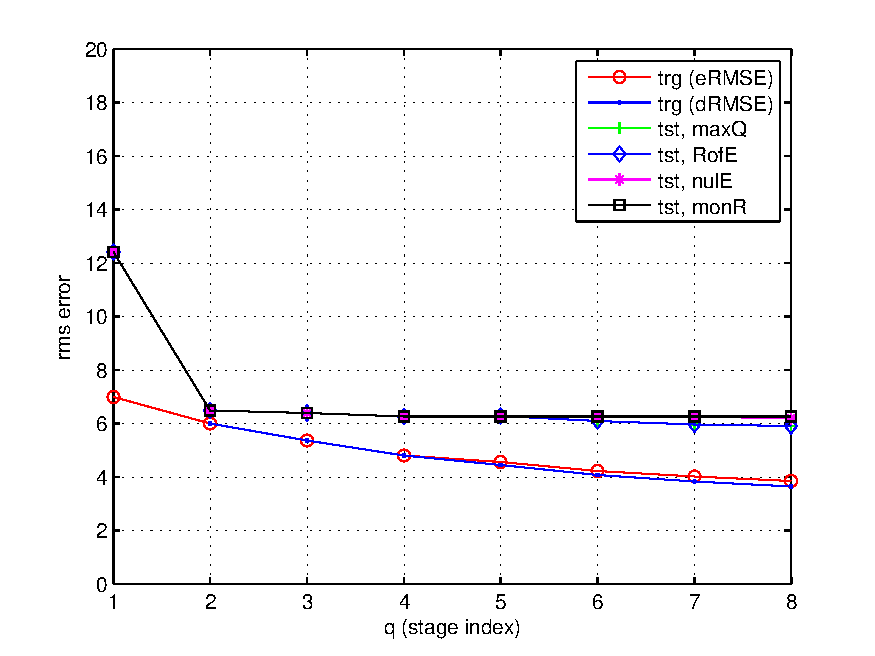
\includegraphics[width=0.45\textwidth]{figs/RVQ_8x4_Dudek_trg_1_to_100_tst_101.pdf}}\hspace{0.2in}
\subfigure[Uniform random variable $U\sim$ \texttt{[}0, 1\texttt{]} in $\mathbb{R}^{1089}$, 100 realizations were used for training.  The test example is a single realization in $\mathbb{R}^{1089}$.]{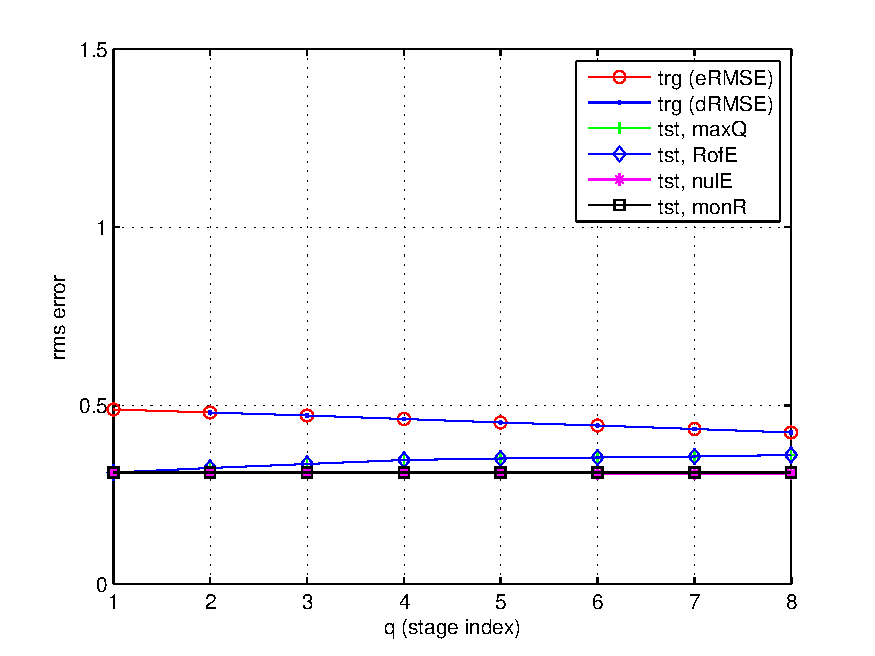
\includegraphics[width=0.45\textwidth]{figs/RVQ_8x4_uniform_trg_100_tst_1.pdf}}
\subfigure[Gaussian random variable $\mathcal{N}\sim$(0, 1) in $\mathbb{R}^{1089}$, 100 realizations were used for training.  The test example is a single realization in $\mathbb{R}^{1089}$.]{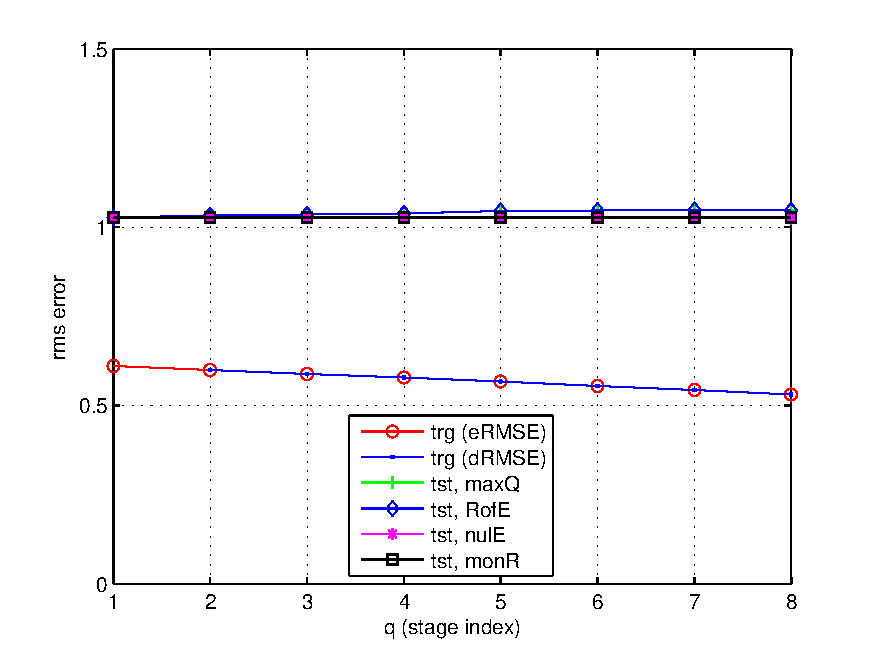
\includegraphics[width=0.45\textwidth]{figs/RVQ_8x4_Gaussian_trg_100_tst_1.pdf}}\hspace{0.55in}
\subfigure[Gauss-Markov random variable $\mathcal{N}\sim$(0, 1) in $\mathbb{R}^{1089}$ with 0.9 correlation, 100 realizations were used for training.  The test example is the 101st realization in $\mathbb{R}^{1089}$ and has correlation with the 100th realization.]{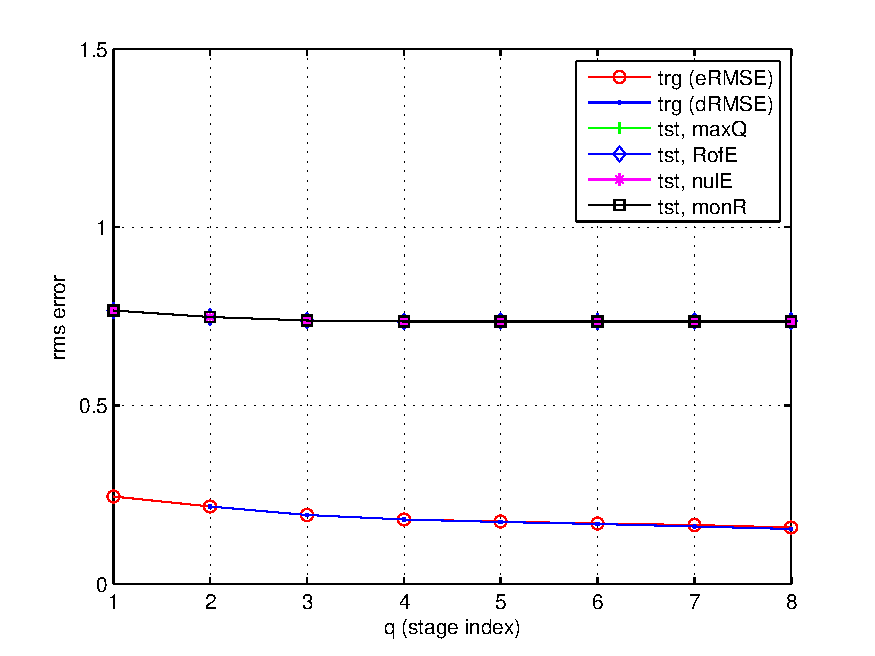
\includegraphics[width=0.45\textwidth]{figs/RVQ_8x4_GaussMarkov_trg_100_tst_1.pdf}}
\caption{RVQ experiments with 8x4 codebook. 100 training examples in $\mathbb{R}^{1089}$ were used for each of these experiments.  A single test example in $\mathbb{R}^{1089}$ was reconstructed.}
\label{fig:RVQ_results}
\end{figure}

%================================
\section{Conclusions}
%================================
In these experiments, we see that as $q$, the number of stages increases, training error and test error decrease.  This is as expected.  However, we intend to do more experiments using cross-validation to gain more confidence in these results.

These initial experiments appear to confirm the fact that RVQ has variable VC dimension.  Whereas it is to be expected that increasing stages will decrease reconstruction error, both at design-time and run-time, ERM (empirical risk minimization) from statistical learning theory can be used as a justification for the number of stages $q$ that are used in a given classification or tracking scenario.


\clearpage
\newpage
\normalsize
\bibliographystyle{ieee}
\bibliography{MyCitations}
\end{document}